% !TeX encoding = UTF-8



\documentclass[11pt,a4paper]{article}

\usepackage[top=1.8cm, left=2cm, bottom=1.8cm, text={17cm, 24cm}]{geometry}
\usepackage[slovak]{babel}
\usepackage[utf8]{inputenc}
\usepackage[T1]{fontenc}
\usepackage{lmodern}
\usepackage{courier}
\usepackage{mathpazo}
\usepackage{eulervm}
\usepackage{cmap}

\usepackage{graphicx}
\usepackage{caption}
\usepackage{subcaption}
\usepackage{smartdiagram}
\usepackage{epstopdf}
\usepackage{url}
\usepackage{breakurl}
\usepackage[breaklinks,hidelinks]{hyperref}
\usepackage{amsmath}
\usepackage{amsfonts}
\usepackage{gensymb}
\usepackage{bm}
\usepackage{blindtext}
\usepackage{listings}
\usepackage{color}
\usepackage{enumitem}
\usepackage{tikz}
\usetikzlibrary{graphs,	graphs.standard}
\usepackage{tkz-berge}
\usepackage{pgfplots}
\pgfplotsset{compat=1.5}

\hypersetup{breaklinks=true}
\urlstyle{same}

\usepackage{xcolor}
\hypersetup{
	colorlinks,
	linkcolor={red!50!black},
	citecolor={blue!50!black},
	urlcolor={blue!80!black}
}

\pgfplotsset{mystyle/.style={%
	%	tick label style = {font=\sansmath\sffamily},
		width=13cm,
		height=5.5cm,
		ylabel={Čas [s]},
		xlabel={Počet radených prvkov},
		xmin=0,xmax=70,
		xtick={0,2,4,8,16,32,64},
		tick style={semithick},
		y tick label style={
		 	/pgf/number format/.cd,
		 	fixed,
		 	fixed zerofill,
		 	precision=2,
		 	/tikz/.cd
		 },
		%font=\sffamily,
		%every axis label/.append style={font=\sffamily},
		%tick label style={font=\sffamily},
	}
}

\definecolor{codegreen}{rgb}{0,0.6,0}
\definecolor{codegray}{rgb}{0.5,0.5,0.5}
\definecolor{codepurple}{rgb}{0.58,0,0.82}
\definecolor{backcolour}{rgb}{0.95,0.95,0.92}

\lstdefinestyle{mystyle}{
	backgroundcolor=\color{backcolour},   
	commentstyle=\color{codegreen},
	keywordstyle=\color{magenta},
	numberstyle=\tiny\sffamily\ttfamily\color{codegray},
	stringstyle=\color{codepurple},
	basicstyle=\footnotesize\sffamily\ttfamily,
	breakatwhitespace=false,         
	breaklines=true,                 
	captionpos=b,                    
	keepspaces=true,                 
	numbers=left,                    
	numbersep=5pt,                  
	showspaces=false,                
	showstringspaces=false,
	showtabs=false,                  
	tabsize=4,
}

\lstset{style=mystyle}

\begin{document}
	
\begin{figure}[h]

\includegraphics[scale=0.35]{FIT_barevne_PANTONE_CZ.eps}
\end{figure}


\noindent \textbf{\Large{Měření RIP count}  (počet papilárních linií)} \\ 
Dokumentácia k projektu do predmetu BIO

\vspace{0.5cm}

\noindent\begin{tabular}{@{}lll}
Autor:  &\textbf{Marek Milkovič} & \texttt{xmilko01}\\
  &\textbf{Oliver Nemček} & \texttt{xnemce03} \\
Dátum:  & \today
\end{tabular}

\section*{Úvod}
Táto dokumentácia popisuje implementáciu programu, ktorého cieľom je určiť počet papilárnych línií na obrázku odtlačku prsta. Zadanie nekladie špecifické požiadavky na formu a spracovanie projektu. Vzhľadom na povahu projektu sme sa rozhodli vytvoriť GUI rozhranie pre užívateľa. V~rozhraní sa bude dať vyznačiť úsečka pomocou myši. Dva koncové body úsečky budú interpretované ako vstupné body od užívateľa, medzi ktorými sa bude určovať počet papilárnych línií.

\section*{Úvod do problematiky}
Pre zistenie počtu papilárnych línií v obrázku odtlačku prsta je nutné vykonať niekoľko transformácií, ktoré vylepšujú kvalitu pôvodného obrázka. To je problém, s ktorým sa musia vysporiadať všetky metódy založené sa zisťovaní dát z obrazových dát. Častý problém je šum alebo fragmentované papilárne línie. Najčastejšou schémou úpravy odtlačku prsta je určenie poľa orientácií(Orientation Field). Následne sa aplikuje vhodne natočený Gaborov filter. Potom sa dáta binarizujú. Výstupným obrazom z preprocesingu je binarizovaný obraz odtlačku prsta. Táto schéma je popísaná v mnohých publikáciách a článkoch \cite{hong, thai} a nazýva sa preprocesing alebo Image Enhancement. Určenie počtu papilárnych línií v zbinarizovanom obrázku je potom triviálne. Všetky fázy preprocesingu a algoritmus určenia metriky RIP count budú uvedené v tomto dokumente.

Zdrojom informácií sa pre nás stali dva články, ktoré popisujú podobné metódy preprocesingu\cite{hong, thai}. Okrem toho sme sa inšpirovali metódou vytvorenia poľa orientácií z knihy \cite{kniha}

\section*{Vstupný obraz}
\begin{figure}[h]
	\centering
	\begin{subfigure}{0.25\textwidth}
		\centering
		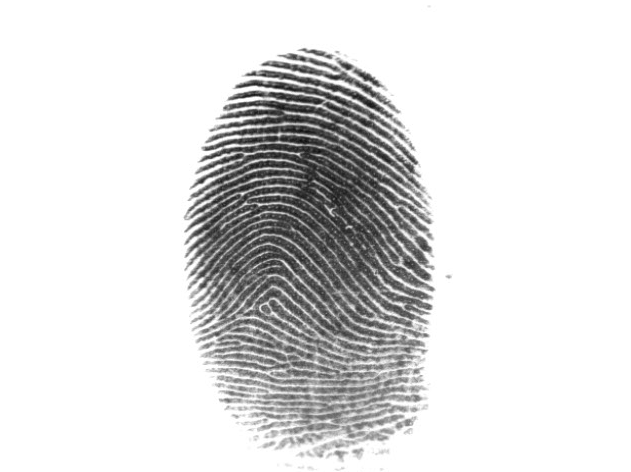
\includegraphics[width=.95\linewidth]{images/Screenshot_1}
	\end{subfigure}%
	\begin{subfigure}{0.25\textwidth}
		\centering
		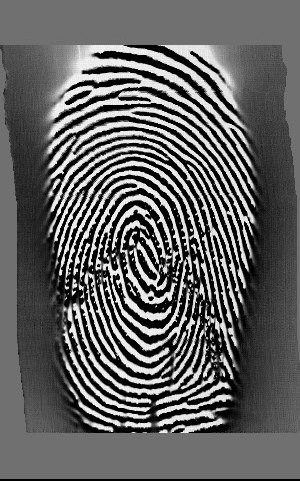
\includegraphics[width=.95\linewidth]{images/Screenshot_2}
	\end{subfigure}%
	\begin{subfigure}{0.25\textwidth}
		\centering
		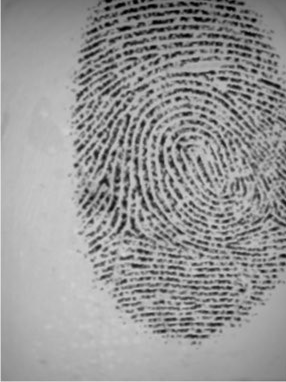
\includegraphics[width=.95\linewidth]{images/Screenshot_3}
	\end{subfigure}%
	\begin{subfigure}{0.25\textwidth}
	\centering
	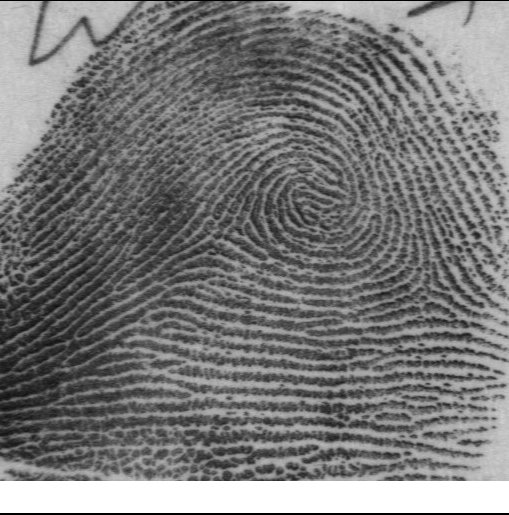
\includegraphics[width=.95\linewidth]{images/Screenshot_4}
\end{subfigure}%
	\caption{Vstupné obrázky odtlačku prsta z rôznych databáz}
	\label{fig:1}
\end{figure}

V priebehu vývoja sme čerpali vstupné dáta výlučne z verejných databáz, ktoré sú dostupné na internete. Kvôli vyššej diverzite sme sa rozhodli využiť niekoľko databáz, ktoré sa nám podarilo stiahnuť. Všetky odkazy sú uvedené v závere tejto práce. Problémom vstupných súborov je dramaticky odlišná kvalita jednotlivych obrázkov, obrázok \ref{fig:1}, nie len z rozdielnych databáz ale aj vrámci jednej databázy. Okrem toho, niektoré obrázky sú nasnímané použitím iných senzorov, čo priamo ovplyvňuje charaketristiku obrázka. Vo preprocesingu musíme zvoliť vhodné hodnoty parametrov pre daný obrázok a zaistiť tak aby bola kvalita výstupu čo najvýššia. Rozhodli sme sa nechať užívateľovi možnosť priamo nastaviť jeden parameter, ktorý sa mení vzhľadom na vstupnú charakteristiku obrázka -- prah variancie. Tento parameter slúži k separácii pozadia a popredia v obrázku.

\section*{Preprocesing}
Vrámci preprocesingu sme sa rozhodli vykonať úpravu rozmerov obrázka tak, aby jeho výška aj šírka boli násobkom 16. Metódou orezania obrázka odstránime najpravejšie prípadne najspodnejšie pixely, podľa vstupných rozmerov. Umožní nám to jednoducho používať blokové transformácie. 
V prípade, že obrázok je farebný, je konvertovaný na čierno-biely podľa štandardných konvencií. Hodnoty pixelov nadobúdajú hodnoty 0--255 a sú uložené v dátovom type \texttt{unsigned char}.

Vylepšenie obrázka sa zkladá z nasledujúcich fáz. Podrobne ich popíšeme:

\subsection*{Segmentácia}
Prvá fáza, ktorú vykonávame na vstupnom obrázku je segmentácia. Jej účelom je odlíšiť pozadie obrázka od popredia. Výstupom je takzvaný ROI(Region Of Interest). Algoritmus pracuje na blokoch o veľkosti 16x16 pixelov. Vychádzame z predpokladu, že na pozadí nedochádza k prudkým zmenám hodnôt pixelov. Ako Metrika zmeny sa používa smerodajná odchylka(v materiáloch sa nazýva aj variancia).

Postup algoritmu je nasledovný:
\begin{enumerate}
	\item Rozdelenie obrazu na samostatné neprekrývajúce sa bloky o veľkosti 16x16 pixelov.
	\item Pre každý blok spočítame hodnotu variancie.
	\item Pokiaľ hodnota variancie je menšia ako prahová hodnota, potom je blok súčasťou pozadia, inak je súčasťou popredia.
\end{enumerate}

Ilustrovaný algoritmus vykazuje dobré výsledky, pokiaľ je popredie dostatočne odlíšené od pozadia. Nastavenie prahu sa ale významne líši a je špecifické pre každý obrázok. Na obrázkoch \ref{fig:2} je červenou farbou označný blok pozadia a zelenou farbou označený blok popredia. Pozorný čítateľ si určite všimne, že v prvom obrázku stačí nastaviť prah variancie na hodnotu 1. Na druhom obrázku je variancia nastavená na 500 aby segmentácia bola dosatočne kvalitná. Na poslednom obrázku je ilustrovaná chyba, kedy sa popredie označí ako pozadie, pretože došlo k pretečeniu čiernej zložky do bielej. V danom prípade sa znížila hodnota variancie bloku pod úroveň prahu.

\begin{figure}[h!]
	\centering
	\begin{subfigure}{0.33\textwidth}
		\centering
		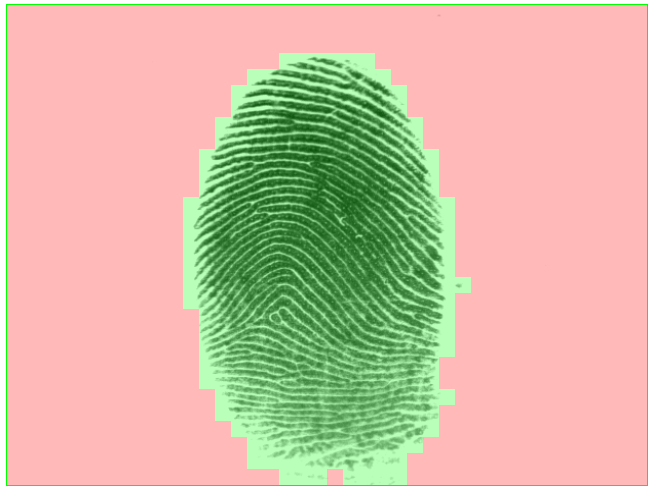
\includegraphics[width=.95\linewidth]{images/Screenshot_5}
		\caption{Hodnota prahu variancie = 1}
		\label{fig:gull}
	\end{subfigure}%
	\begin{subfigure}{0.33\textwidth}
		\centering
		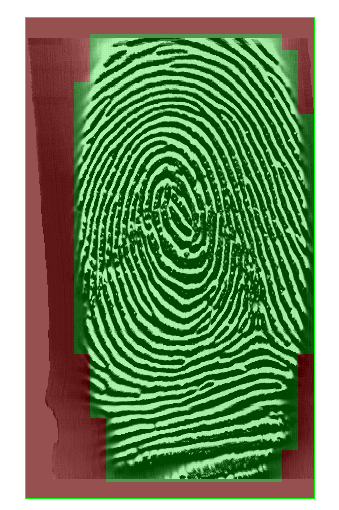
\includegraphics[width=.95\linewidth]{images/Screenshot_6}
		\caption{Hodnota prahu variancie = 500}
		\label{fig:gull2}
	\end{subfigure}%
	\begin{subfigure}{0.33\textwidth}
		\centering
		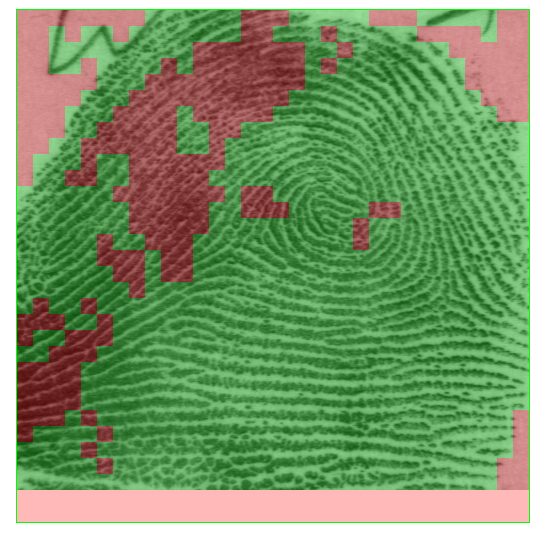
\includegraphics[width=.95\linewidth]{images/Screenshot_7}
		\caption{Hodnota prahu variancie = 500}
		\label{fig:tiger}
	\end{subfigure}%
	\caption{Rôzne hodnoty prahu variancie pre rozne obrázky}\label{fig:2}
\end{figure}

Výstup segmentácie je logická hodnota priradená každému bloku, ktorá popisuje, či je daný blok \uv{zaujímavý}(ROI).








\subsection*{Normalizácia}
Účelom tejto transformácie je vyhladiť rozdiely v kontraste v každej časti obrázku. Niektoré transformácie by vykazovali nestabilné výsleky, pokiaľ by pracovali s obrázkom, v ktorom by sa nachádzali kontrastné rozdiely.
Transformácia by sa dala chápať ako low-pass filter, pretože odstráni vysokofrekvenčné zložky z obrazu.
Popisovaný algoritmus je prebratý z článku \cite{thai}. Algoritmus počíta priemernú hodnotu len z pixelov popredia a aplikuje ich na všetky pixely.

Konštantami pre algoritmus je výsledná priemerná hodnota obrázku $M_0$ a výsledná variancia obrázku označená ako  $V_0$. Podľa článku sme obe hodnoty nastavili na hodnotu 100.

\begin{figure}[h]
	\centering
	\begin{subfigure}{0.50\textwidth}
		\centering
		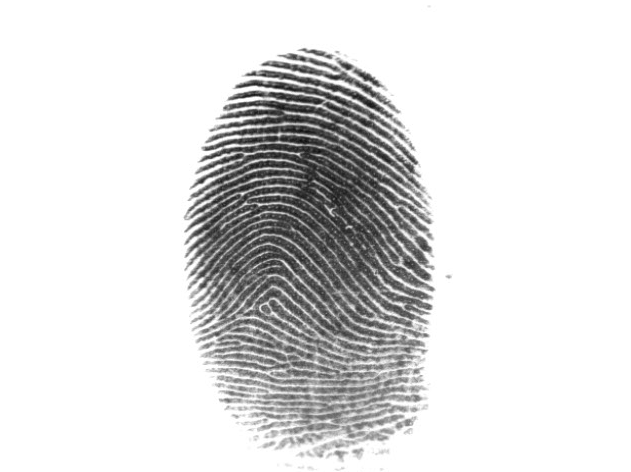
\includegraphics[width=\linewidth]{images/Screenshot_1}
		\caption{Pred normalizáciou}
	\end{subfigure}%
	{\LARGE$\xrightarrow{}$}
	\begin{subfigure}{0.45\textwidth}
		\centering
		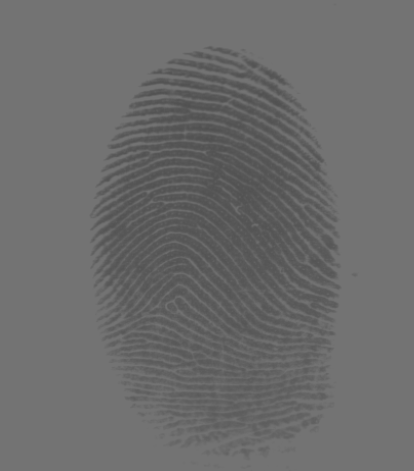
\includegraphics[width=.7\linewidth]{images/Screenshot_8}
		\caption{Po normalizácií}
	\end{subfigure}%
	\caption{Proces normalizácie, $M_0 = V_0 = 100$}\label{fig:3}
\end{figure}

 \begin{equation}
P(x,y) =
\begin{cases}
M_0 \boldsymbol {+} \sqrt{\frac{V_0 \cdot (I(x,y) -M )^2 }{V}}, & \text{ak}\ I(x,y)>M \\
M_0 \boldsymbol {-} \sqrt{\frac{V_0 \cdot (I(x,y) -M )^2 }{V}}, & \text{inak}
\end{cases}
\label{eq:1}
\end{equation}

\begin{enumerate}
	\item Spočítaj priemernú hodnotu a varianciu pre všetky pixely, ktoré patria do popredia.
	\item Pre každý pixel aplikuj rovnicu \ref{eq:1}, kde $P$ je výstupný pixel, $I$ je vstupný pixel, $V_0$ je zvolená variancia, $M_0$ je zvolená priemerná hodnota,  $M$ je priemerná hodnota,  $V$ je variancia.
\end{enumerate}

Výstupom je obrázok ktorý má vyrovnané kontrastné rozdiely a je pripravený na dalšie spracovanie.
Ilustrácia tohoto kroku je na obrázku \ref{fig:3}














\subsection*{Pole orientácií}
Veľmi dôležitou súčasťou retazca transformácií je určenie smeru, v ktorom sa papilárna línia nachádza. V článku \cite{thai} sa uvádza uhol $\Theta$ ako uhol medzi osou X a smerom papilárnej línie, viď obrázok \ref{fig:4}.

\begin{figure}[h]
	\centering
	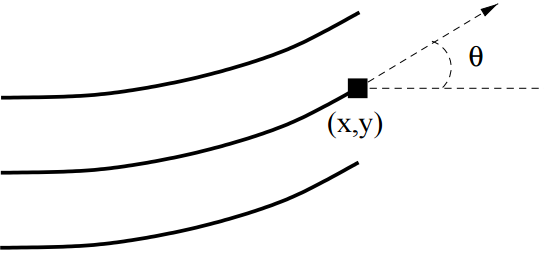
\includegraphics[width=.4\linewidth]{images/Screenshot_9}
	\caption{V poli orientácií je hodnota reprezentovaná uhlom $\Theta$}
	\label{fig:4}
\end{figure}

Princípom tejto transformácie je určenie gradientu o osiach X a Y. Niektoré články riešia problém pomocou rozdelenia obrázku na bloky a počítajú priemerný uhol bloku dát. My sme sa rozhodli vykonávať transformáciu nad každým pixelom, okolo ktorého vytvoríme blok tak, že daný pixel sa nachádza v strede bloku. Vstupom transformácie je normalizovaný obrázok.

Prvým krokom pre získanie poľa orientácií je určenie gradientu(2D derivácie) pre os X a Y pomocou Sobelovho operátora, rovnice \ref{eq:2.1}.
\begin{align}
\begin{split}
D_x &= Sobel(X, image)\\
D_y &= Sobel(Y, image)\\ 
\end{split}
\label{eq:2.1}
\end{align}

Následne pre každý pixel z popredia vytvoríme blok o veľkosti 11x11 pixelov. Na každý pixel z bloku aplikujeme rovnice \ref{eq:2.2}. Súčtom hodnôt zanesieme do výsledku aj orientácie okolitých pixelov. Robíme to kvôli zjemneniu a vyhladeniu výsledku.

\begin{align}
\begin{split}
G_{xy} &+= D_x(x,y) * D_y(x,y)\\
G_{xx} &+= D_x(x,y)^2\\
G_{yy} &+= D_y(x,y)^2\\
\end{split}
\label{eq:2.2}
\end{align}

Nakoniec pre stredový pixel z daného bloku spočítame orientáciu podľa rovnice \ref{eq:2}. Dôležitým prvkom je funkcia \texttt{atan2}, ktorá oproti variante \texttt{atan} správne určí kvadrant(znamienko) výslednej hodnoty.

\begin{align}
\begin{split}
\Theta(x,y) &= 0.5 * (\pi + atan2(2 \cdot G_{xy}, G_{xx} - G_{yy}))
\end{split}
\label{eq:2}
\end{align}




Výhodou tohto výpočtu oproti postupom popísaným v článkoch \cite{hong, thai} je fakt, že hodnoty v poli $\Theta$ netreba ďalej priemerovať alebo vyhladzovať. Smer okolitých pixelov bol zanesený priamo do výpočtu.

Jediným parametrom, ktorý sa môže nastavovať v tejto fáze je veľkosť bloku, nad ktorým sa počítajú hodnoty $G_{xx}, G_{yy}, G_{xy}$. Na základe publikácie \cite{kniha} sme zvolili odporúčanú hodnotu 11x11 pixelov.


\begin{figure}[h!]
	\centering
	\begin{subfigure}{0.42\textwidth}
		\centering
		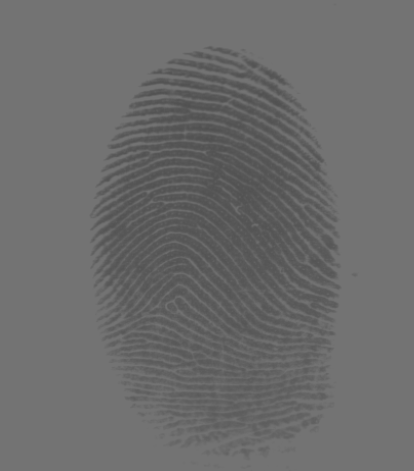
\includegraphics[width=\linewidth]{images/Screenshot_8}
		\caption{Normalizovaný obrázok}
	\end{subfigure}%
	{\LARGE$\xrightarrow{}$}
	\begin{subfigure}{0.45\textwidth}
		\centering
		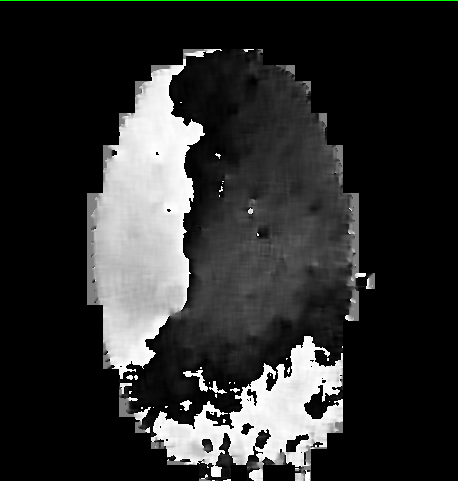
\includegraphics[width=\linewidth]{images/Screenshot_10}
		\caption{Grafická reprezentácia poľa orientácií}
	\end{subfigure}%
	\caption{Vytvorenie poľa orientácií}\label{fig:5}
\end{figure}





\subsection*{Gaborov filter}
Najzaujímavejším a najzložitejším filtrom v reťazci je Gaborova filtrácia. Princípom je dvojrozmerná konvolúcia bloku dát normalizovaného obrázka s vhodne natočeným Gaborovým filtrom. Najdôležitejšou vlastnosťou filtra z pohľadu odtlačkov prstov je schopnosť zvýrazniť papilárne línie a významne potlačiť šum spolu s drobnými fragmentáciami. 

\begin{figure}[h!]
	\centering
	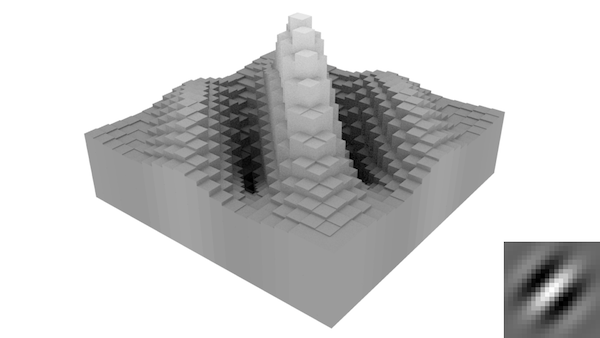
\includegraphics[width=.4\linewidth]{images/gabor_kernel}
	\caption{3D reprezentácia Gaborovho filtra pod uhlom 45$\degree$}
	\label{fig:7}
\end{figure}

\begin{figure}[h!]
	\centering
	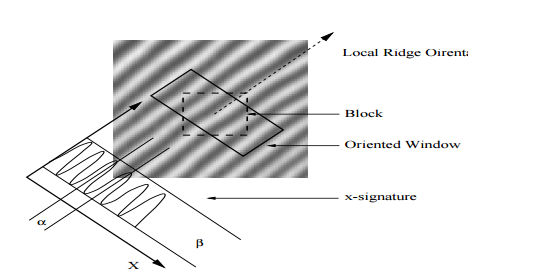
\includegraphics[width=.7\linewidth]{images/Screenshot_11}
	\caption{Vytvorenie orientovaného okna, \cite{hong}}
	\label{fig:6}
\end{figure}

Z hľadiska spracovania signálov je gaborov filter Gaussovská pásmová priepusť. Modulovacia funkcia je sinus, prípadne kosínus. Vzhľadom na základ filtra v Gausovej distribučnej funkcii je nutné zvoliť parameter $\sigma$. V dokumente \cite{hong} je zvolená hodnota $\sigma_x = \sigma_y = 4$. Čím vyššia je hodnota $\sigma$ tým viac sa do výslednej hodnoty primiešava hodnota okolitých pixelov.


V predošlej fáze sme zistili pre každý pixel orientáciu papilárnej línie. Gaborov filter môžeme teda natočiť požadovaným smerom. Modulačná frekvencia je dôležitým parametrom filtra, zlé nastavenie frekvencie môže mať významný vplyv na kvalitu výstupného obrázku. 

Určenie frekvencie(vzdialenosti mezi dvoma vrcholmi) robíme podobne ako v práci \cite{hong}. Pre každý pixel vytvoríme orientované okno s veľkosťou 32x16(dĺžka, šírka) pixelov so stredom v danom pixeli, viď obrázok \ref{fig:7}. Po vytvorení okna prichádza na rad priemerovanie hodnôt cez šírku okna. Výstupom je okno s veľkosťou 32x1 pixelov, ktoré interpretujeme ako 1D signál podobný sinusoidu. Určenie vzdialenosti medzi dvomi vrcholmi vykonávame na základe našej vlastnej metódy. Najprv spočítame FFT nad 1D signálom. Potom jednotlivé zastúpenia modulov frekvencií spočítame váženým priemerom(súčin veľkosti modulu frekvencie a frekvencie). Maximálna frekvencia je nastavená na 11 kmitov. 

Odhadovaná frekvencia a smer sú použité na konštrukciu Gaborovho filtra pre daný pixel. Postup je nasledovný:

\begin{enumerate}
	\item Pre každý pixel z popredia vytvor orientované okno a spočítaj frekvenciu(priemernú vzdialenosť vrcholov v okne).
	\item Okolo daného pixelu vytvor blok s veľkosťou 18x18 pixelov.
	\item Vytvor Gaborov filter s veľkosťou 18x18 pixelov, s daným smerom a frekvenciou.
	\item Aplikuj konvolúciu bloku s Gaborovým filtrom, opužitý operátor je násobenie.
	\item Hodnota výstupného pixelu je priemerná hodnota konvolvovaného bloku.
\end{enumerate}

Správnym nastavením Gaborovho filtra je možné extrahovať papilárne línie aj z menej  kvalitného vstupu.


\begin{figure}[h!]
	\centering
	\begin{subfigure}{0.3\textwidth}
		\centering
		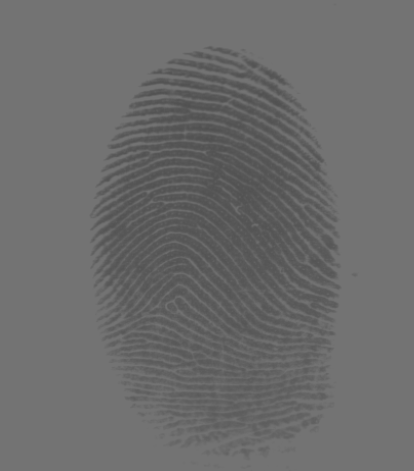
\includegraphics[width=.95\linewidth]{images/Screenshot_8}
		\caption{Normalizovaný obrázok}
	\end{subfigure}%
	{\LARGE$+$}
	\begin{subfigure}{0.3\textwidth}
		\centering
		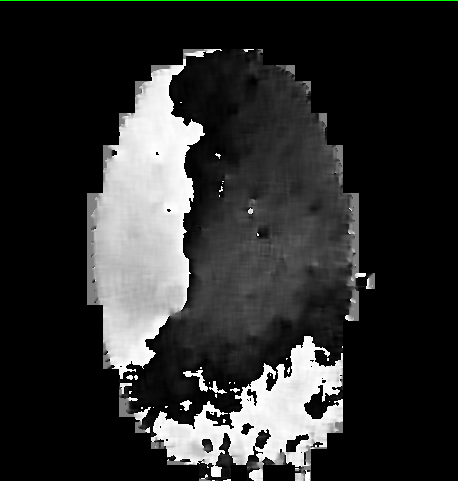
\includegraphics[width=\linewidth]{images/Screenshot_10}
		\caption{Pole orientácií}
	\end{subfigure}%
	{\LARGE$\xrightarrow{}$}
	\begin{subfigure}{0.3\textwidth}
		\centering
		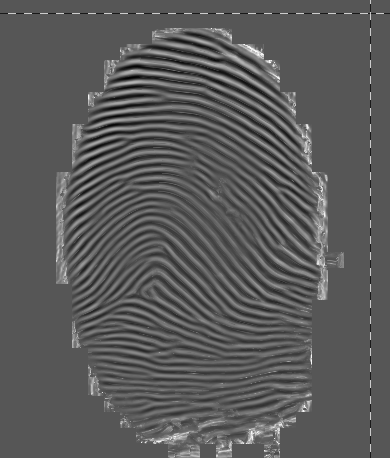
\includegraphics[width=.95\linewidth]{images/Screenshot_12}
		\caption{Gaborova filtrácia}
	\end{subfigure}%
	\caption{Ilustrácia Gaborovho filtra}\label{fig:8}
\end{figure}

\subsection*{Binarizácia}
Posledným dielom v sústave filtrov je binarizácia. Jej úloha je triviálna. Mapuje výstup z Gaborovho filtra na hodnoty 0 alebo 255. Postup je nasledovný:
\begin{enumerate}
	\item Pre každý pixel z výstupu Gaborovho filtra aplikuj nasledovnú rovnicu
	\item Ak je hodnota pixelu väčšia ako 0, potom priraď 255, inak 0.
\end{enumerate}

\begin{figure}[h!]
	\centering
	\begin{subfigure}{0.45\textwidth}
		\centering
		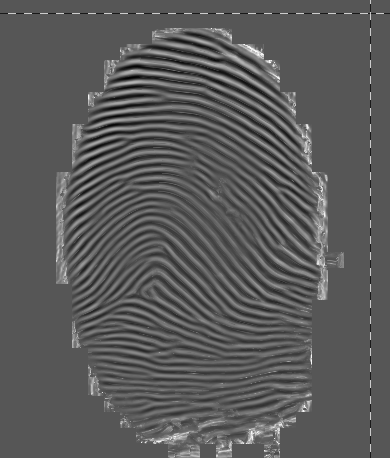
\includegraphics[width=.95\linewidth]{images/Screenshot_12}
		\caption{Výstup z Gaborovho filtra}
	\end{subfigure}%
	{\LARGE$\xrightarrow{}$}
	\begin{subfigure}{0.40\textwidth}
		\centering
		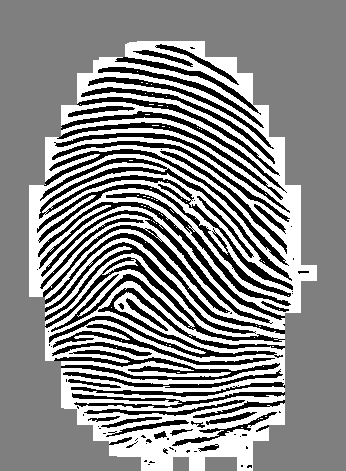
\includegraphics[width=.95\linewidth]{images/Screenshot_13}
		\caption{Binarizácia}
	\end{subfigure}%
	\caption{Ilustrácia binarizácie}\label{fig:9}
\end{figure}

Výstupom binarizácie je čierno-biely obrázok.

\section*{Počítanie RIP count}
Počítanie papilárnych línií spočiva v definovaní dvoch krajných bodov. Potom sa vyvzorkuje binarizovaný obrázok mezi týmito dvomi bodmi. Následne sa spočítajú úseky, ktoré majú hodnotu 0. Neaplikujú sa žiadne ďalšie heuristiky.

Táto fáza je jednoduchá vzhľadom na to, že preprocesing obrázka by mal dostatočne zvýšiť jeho kvalitu.

Výstupom je číslo reprezentujúce počet línií medzi dvoma bodmi. Toto číslo sa zobrazuje v GUI.

\section*{Štatistika}
Maximálny počet papilárnych línii v smere osi Y je zobrazovaný v GUI programu a počíta sa rovnakým algoritmom ako v prípade užívateľsky zvolených bodov. Program vytvorí všetky vertikálne čiary a spočíta k nim RIP count metriku. Maximálnu hodnotu línií zobrazí spolu s čiarou označujúcou miesto s maximálnym počtom línií.


\section*{GUI}
Vzhľadom na povahu projektu sme sa už na začiatku rozhodli umožniť užívateľovi grafickou cestou vyznačiť dva body, medzi ktorými dôjde k spočítaniu papilárnych línií. Tieto dva body sme preložili čiarou s kontrastnou farbou. 
Jednoduché gui s načítaným obrázkom sa nachádza na obrázku \ref{fig:10}.
\begin{figure}[h!]
	\centering
	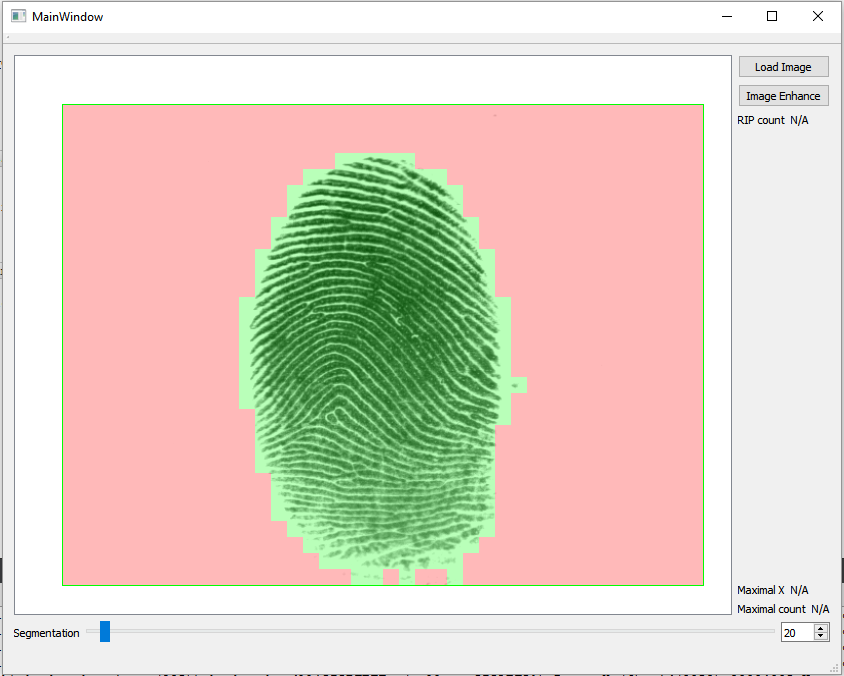
\includegraphics[width=.7\linewidth]{images/Screenshot_14}
	\caption{Hlavné GUI}
	\label{fig:10}
\end{figure}

Po spustení programu sa zobrazí hlavné okno. Užívateľ načíta obrázok kliknutím na tlačidlo \texttt{Load Image}. Zobrazí sa štandardný dialóg operačného systému pre výber súboru. Potom sa obrázok zobrazí v GUI. Nasleduje fáza segmentácie. V dolnej časti GUI sa nachádza horizontálny posúvač spolu s malým oknom zobrazujúcim aktuálnu hodnotu prahu variancie. Užívateľ môze meniť prah a dynamicky s tým dochádza k prekresľovaniu obrázka. Zelená farba označuje popredie, červená pozadie.

Ak je užívateľ spokojný s nastavením segmentačného prahu môže spustiť fázu preprocesigu. K zahájeniu dôjde pri  stlační tlačidla \texttt{Image Enhance}. Po malej chvíli sa zobrazí v GUI binarizovaný obrázok, viď obrázok \ref{fig:11}. 

\begin{figure}[h!]
	\centering
	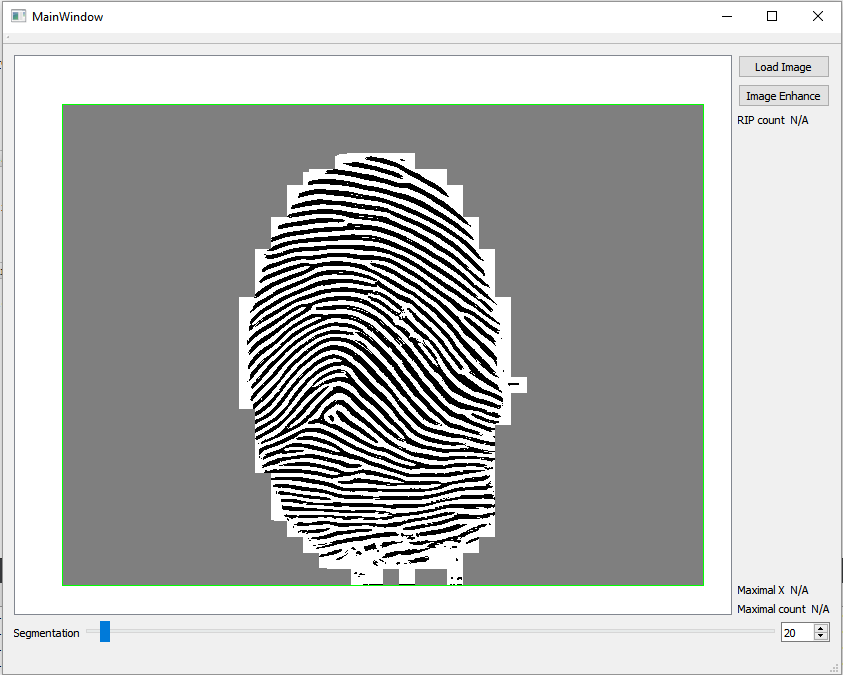
\includegraphics[width=.7\linewidth]{images/Screenshot_15}
	\caption{Hlavné GUI s binarizovaným obrázkom}
	\label{fig:11}
\end{figure}

Do tohoto obrázku už užívateľ môže nakresliť čiaru podobne ako v grafickom editore. Počet papilárnych línií pod čiarou sa zobrazí na pravej strane GUI pri popisku \texttt{RIP count}. Koliečkom myši môže užívateľ obrázok priblížiť/oddialiť. Pri držaní pravého tlačítka myši a jej pohybovaním dochádza k posuvu obrázka(tzv. Drag Mode). Naším cieľom bolo zabezpečiť komfortné ovládanie programu.

\begin{figure}[h!]
	\centering
	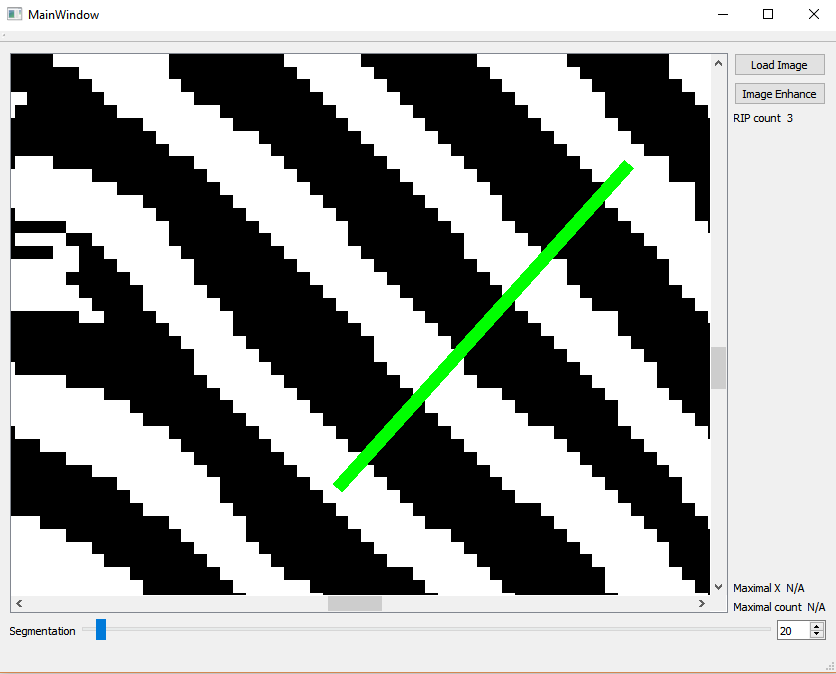
\includegraphics[width=.7\linewidth]{images/Screenshot_16}
	\caption{Zobrazenie metriky RIP count}
	\label{fig:11}
\end{figure}

\section*{Použité technológie}
\begin{itemize}
	\item Qt framework 5.4.0 - multiplatformné GUI
	\item CImg - knižnica pre prácu s obrázkami
\end{itemize}

\section*{Kompilácia}
V archíve sa nachádza kompletný projekt pre Qt Creator. Manuálna kompilácia je možná s použitím knižníc Qt a programom \texttt{qmake}.

\pagebreak

\section*{Záver}
Cieľom projektu bolo vytvoriť program pre zobrazovanie počtu papilárnych línií v zvolenom obrázku odtlačku prsta. Rozhodli sme sa najprv extrahovať papilárne línie zo vstupného obrázku pomocou série filtrácií. Následne určíme počet papilárnych línií medzi dvoma bodmi v binarizovanom obrázku. 

Pre vyšší užívateľský komfort sme pripravili jednoduché GUI, ktoré dovoľuje načítať obrázok v rôznych formátoch. Užívateľ môže obrázkom pohybovať, priližovať a pomocou myši do neho nakresliť čiaru. Program sa postará o výpočet a zobrazenie počtu papilárnych línií.

\pagebreak
\section*{Databázy}
\begin{itemize}
	\item \url{http://bias.csr.unibo.it/fvc2000/Downloads/DB2_B.zip}
	\item \url{http://bias.csr.unibo.it/fvc2004/Downloads/DB1_B.zip}
	\item \url{http://bias.csr.unibo.it/fvc2004/Downloads/DB3_B.zip}
	\item \url{http://bias.csr.unibo.it/fvc2004/Downloads/DB4_B.zip}
	\item \url{http://biosecure.it-sudparis.eu/AB/media/files/samples/fingerprint-ds2-ds3.zip}
	\item \url{http://www.advancedsourcecode.com/PNGfingerprint.rar}
	\item \url{https://s3.amazonaws.com/nist-srd/SD4/NISTSpecialDatabase4GrayScaleImagesofFIGS.zip}
\end{itemize}

\begin{thebibliography}{9}
	\bibitem{hong}
	Hong, Lin et. al. Fingerprint Image Enhancement: Algorithm and Performance Evaluation. Dostupné také z: \url{http://www.math.tau.ac.il/~turkel/imagepapers/fingerprint.pdf}
	\bibitem{thai}
	THAI, Raymond.Fingerprint Image Enhancement and	Minutiae Extraction. Dostupné také z: \url{http://citeseerx.ist.psu.edu/viewdoc/download?doi=10.1.1.121.9756&rep=rep1&type=pdf}
	
	\bibitem{kniha}
	Maltoni, D., Maio, D., Jain, A., Prabhakar, S., Handbook of Fingerprint Recognition.ISBN 978-1-84882-254-2. Dostupné také z: \url{http://link.springer.com/content/pdf/10.1007%2Fb97303.pdf}
\end{thebibliography}


\section*{Poznámky}
V obrázkoch GUI nie je zobrazovaná čiara označujúca miesto s maximálnym počtom papilárnych línií. V čase písania dokumentácie táto funkcionalita nebola dokončená. Vo finálnom produkte sa zobrazuje modrá čiara v mieste s maximálnym počtom papilárnych línií.

\end{document}